\chapter{Introduzione}

L'intelligenza artificiale ha aperto nuove frontiere nella gestione dei segnali biomedici. Sistemi basati su architetture di segmentazione come la U-Net sono oggi in grado di riconoscere tracciati ECG su carta e riconvertirli in segnali numerici. Tuttavia, per essere efficaci, questi modelli richiedono una fase di addestramento basata su una vasta quantità di immagini che simulino le imperfezioni del mondo reale.

\section{Inquadramento del problema}
La digitalizzazione automatica degli ECG richiede un processo di ricostruzione del segnale capace di isolare l'attività elettrica del cuore da elementi di disturbo quali griglie millimetrate, pieghe della carta e macchie di inchiostro. La capacità di generalizzazione dei modelli di Deep Learning dipende interamente dalla varietà dei dati su cui vengono allenati; senza un dataset che includa campioni \textbf{difficili} e deteriorati, le performance su documenti clinici reali rimangono limitate.

\section{Obiettivo del lavoro: Generazione Sintetica e Segmentazione}
Il presente lavoro propone una pipeline a due stadi per la digitalizzazione di immagini ECG. Il primo stadio si focalizza sulla \textbf{generazione sintetica} di immagini ECG realistiche: partendo da un dataset di segnali digitali preesistente, il framework trasforma i dati numerici in rappresentazioni visuali sottoponendole a una pipeline di degradazione controllata, producendo coppie immagine degradata / ground truth binaria. Il secondo stadio sfrutta queste coppie per addestrare un modello di \textbf{segmentazione semantica} capace di isolare i tracciati del segnale da griglia, artefatti e sfondo nelle immagini reali.

\subsection{Integrazione di Artefatti per la Robustezza}
Un contributo centrale risiede nella creazione di un sistema di \textit{data augmentation} avanzato che alimenta direttamente il training del segmentatore. Come dimostrato da Li et al.~\cite{li2020deep}, l'esposizione del modello a disturbi strutturali durante il training è fondamentale per superare il \textit{domain gap} tra i dati sintetici e le scansioni reali, permettendo di incrementarne la robustezza.

\section{Struttura della tesi}
L'elaborato descrive lo sviluppo e la logica del sistema di trasformazione:
\begin{itemize}
    \item \textbf{Capitolo 2:} Descrizione dell'architettura del software e logica di rendering.
    \item \textbf{Capitolo 3:} Analisi della pipeline di artefatti e gestione della varietà del dataset prodotto.
    \item \textbf{Capitolo 4:} Risultati ottenuti e configurazione sperimentale.
    \item \textbf{Capitolo 5:} Modulo di estrazione del segnale ECG tramite segmentazione semantica: architettura del modello, curriculum learning e pipeline di addestramento.
\end{itemize}



\section{Processo di Trasformazione Immagine}
La pipeline si articola in due stadi principali: la conversione del segnale in immagine e l'iniezione controllata di artefatti. Le \textbf{figure \ref{fig:raw_data}, \ref{fig:clean_plot} e \ref{fig:augmented_plot}} mostrano visivamente il processo: partendo dal segnale digitale grezzo, il modulo di rendering produce una rappresentazione grafica, sulla quale vengono applicati i disturbi per simulare le condizioni di conservazione e scansione dei documenti clinici.

\begin{figure}[htbp]
    \centering
    \footnotesize
    \texttt{
    89ff c9ff 4000 5600 \\
    a5ff 0400 bbff e1ff \\
    0000 e6ff d9ff b1ff \\
    8cff cdff 4100 5300 \\
    a6ff 0600 c0ff dcff \\
    fdff e1ff deff b6ff \\
    88ff d4ff 4c00 5200 \\
    9eff 1000 c6ff deff \\
    f6ff e4ff e3ff bbff \\
    8bff daff 5000 4d00 \\
    \ldots
    }
    \caption{Dato grezzo: snippet esadecimale estratto dal dataset ECG.}
    \label{fig:raw_data}
\end{figure}

\begin{figure}[htbp]
    \centering
    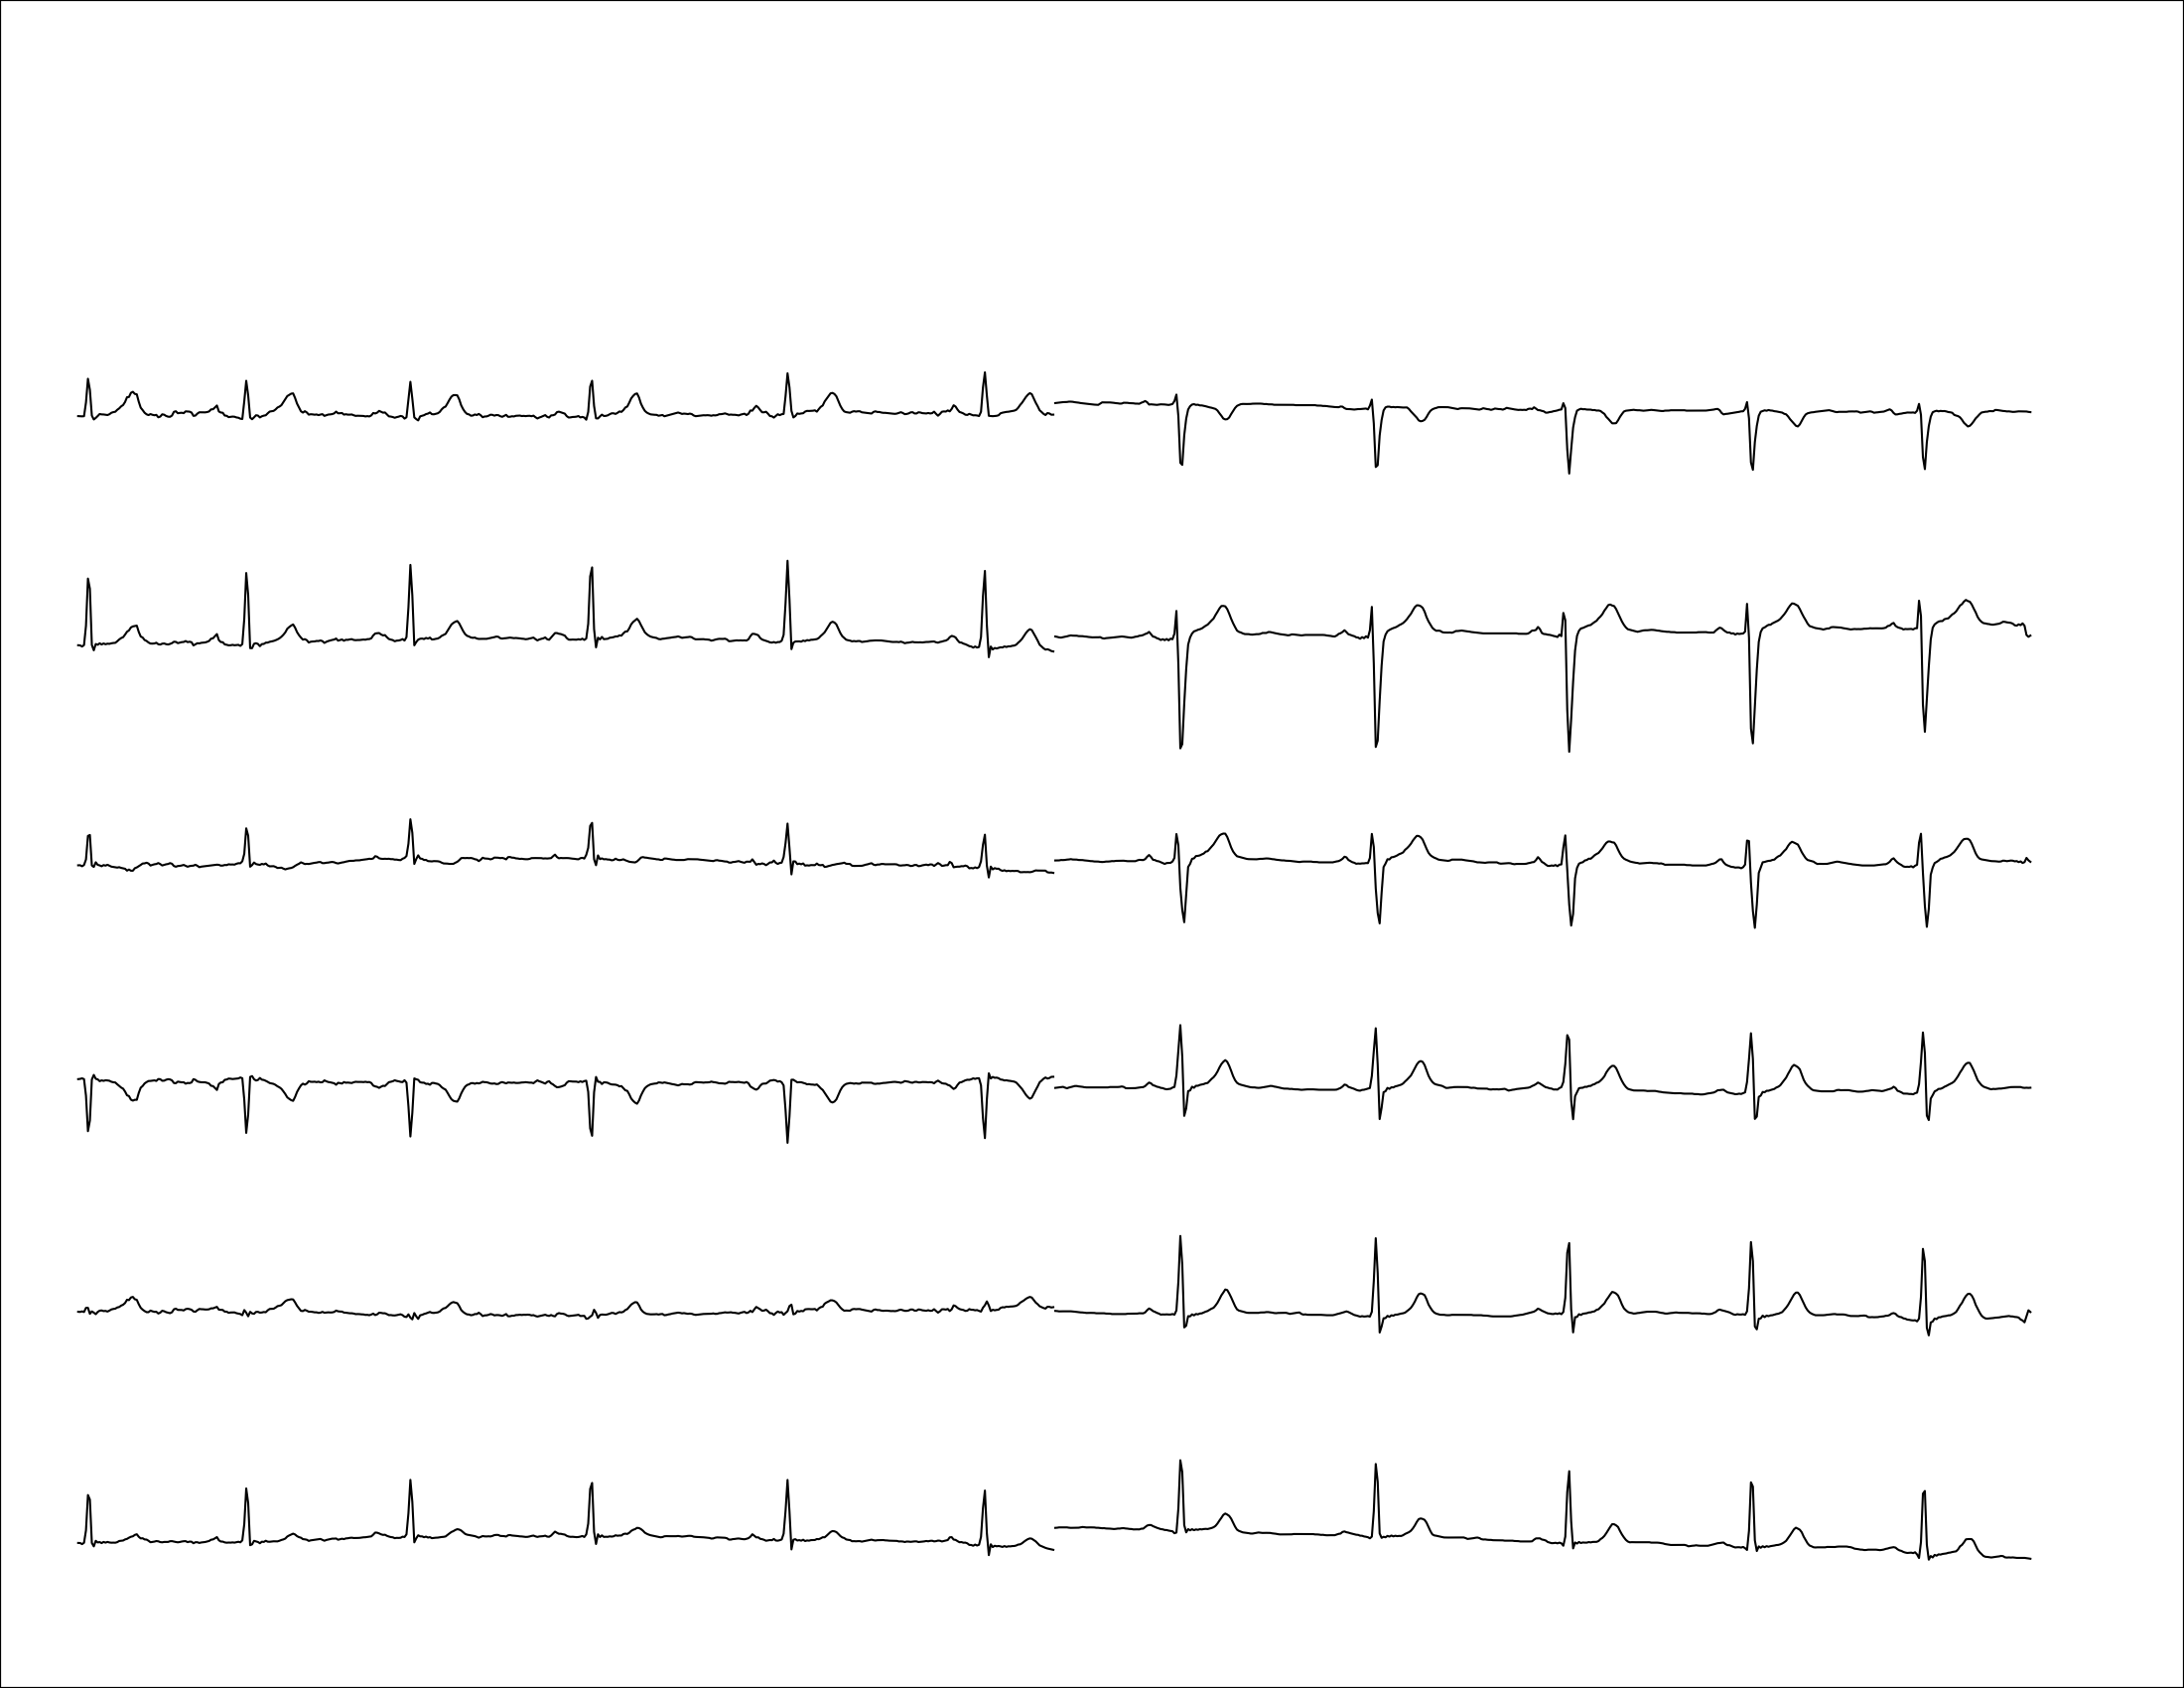
\includegraphics[width=0.7\textwidth, keepaspectratio]{images/clean_plot.png}
    \caption{Visualizzazione su canvas del segnale ECG: tracciato vettoriale pulito.}
    \label{fig:clean_plot}
\end{figure}

\begin{figure}[htbp]
    \centering
    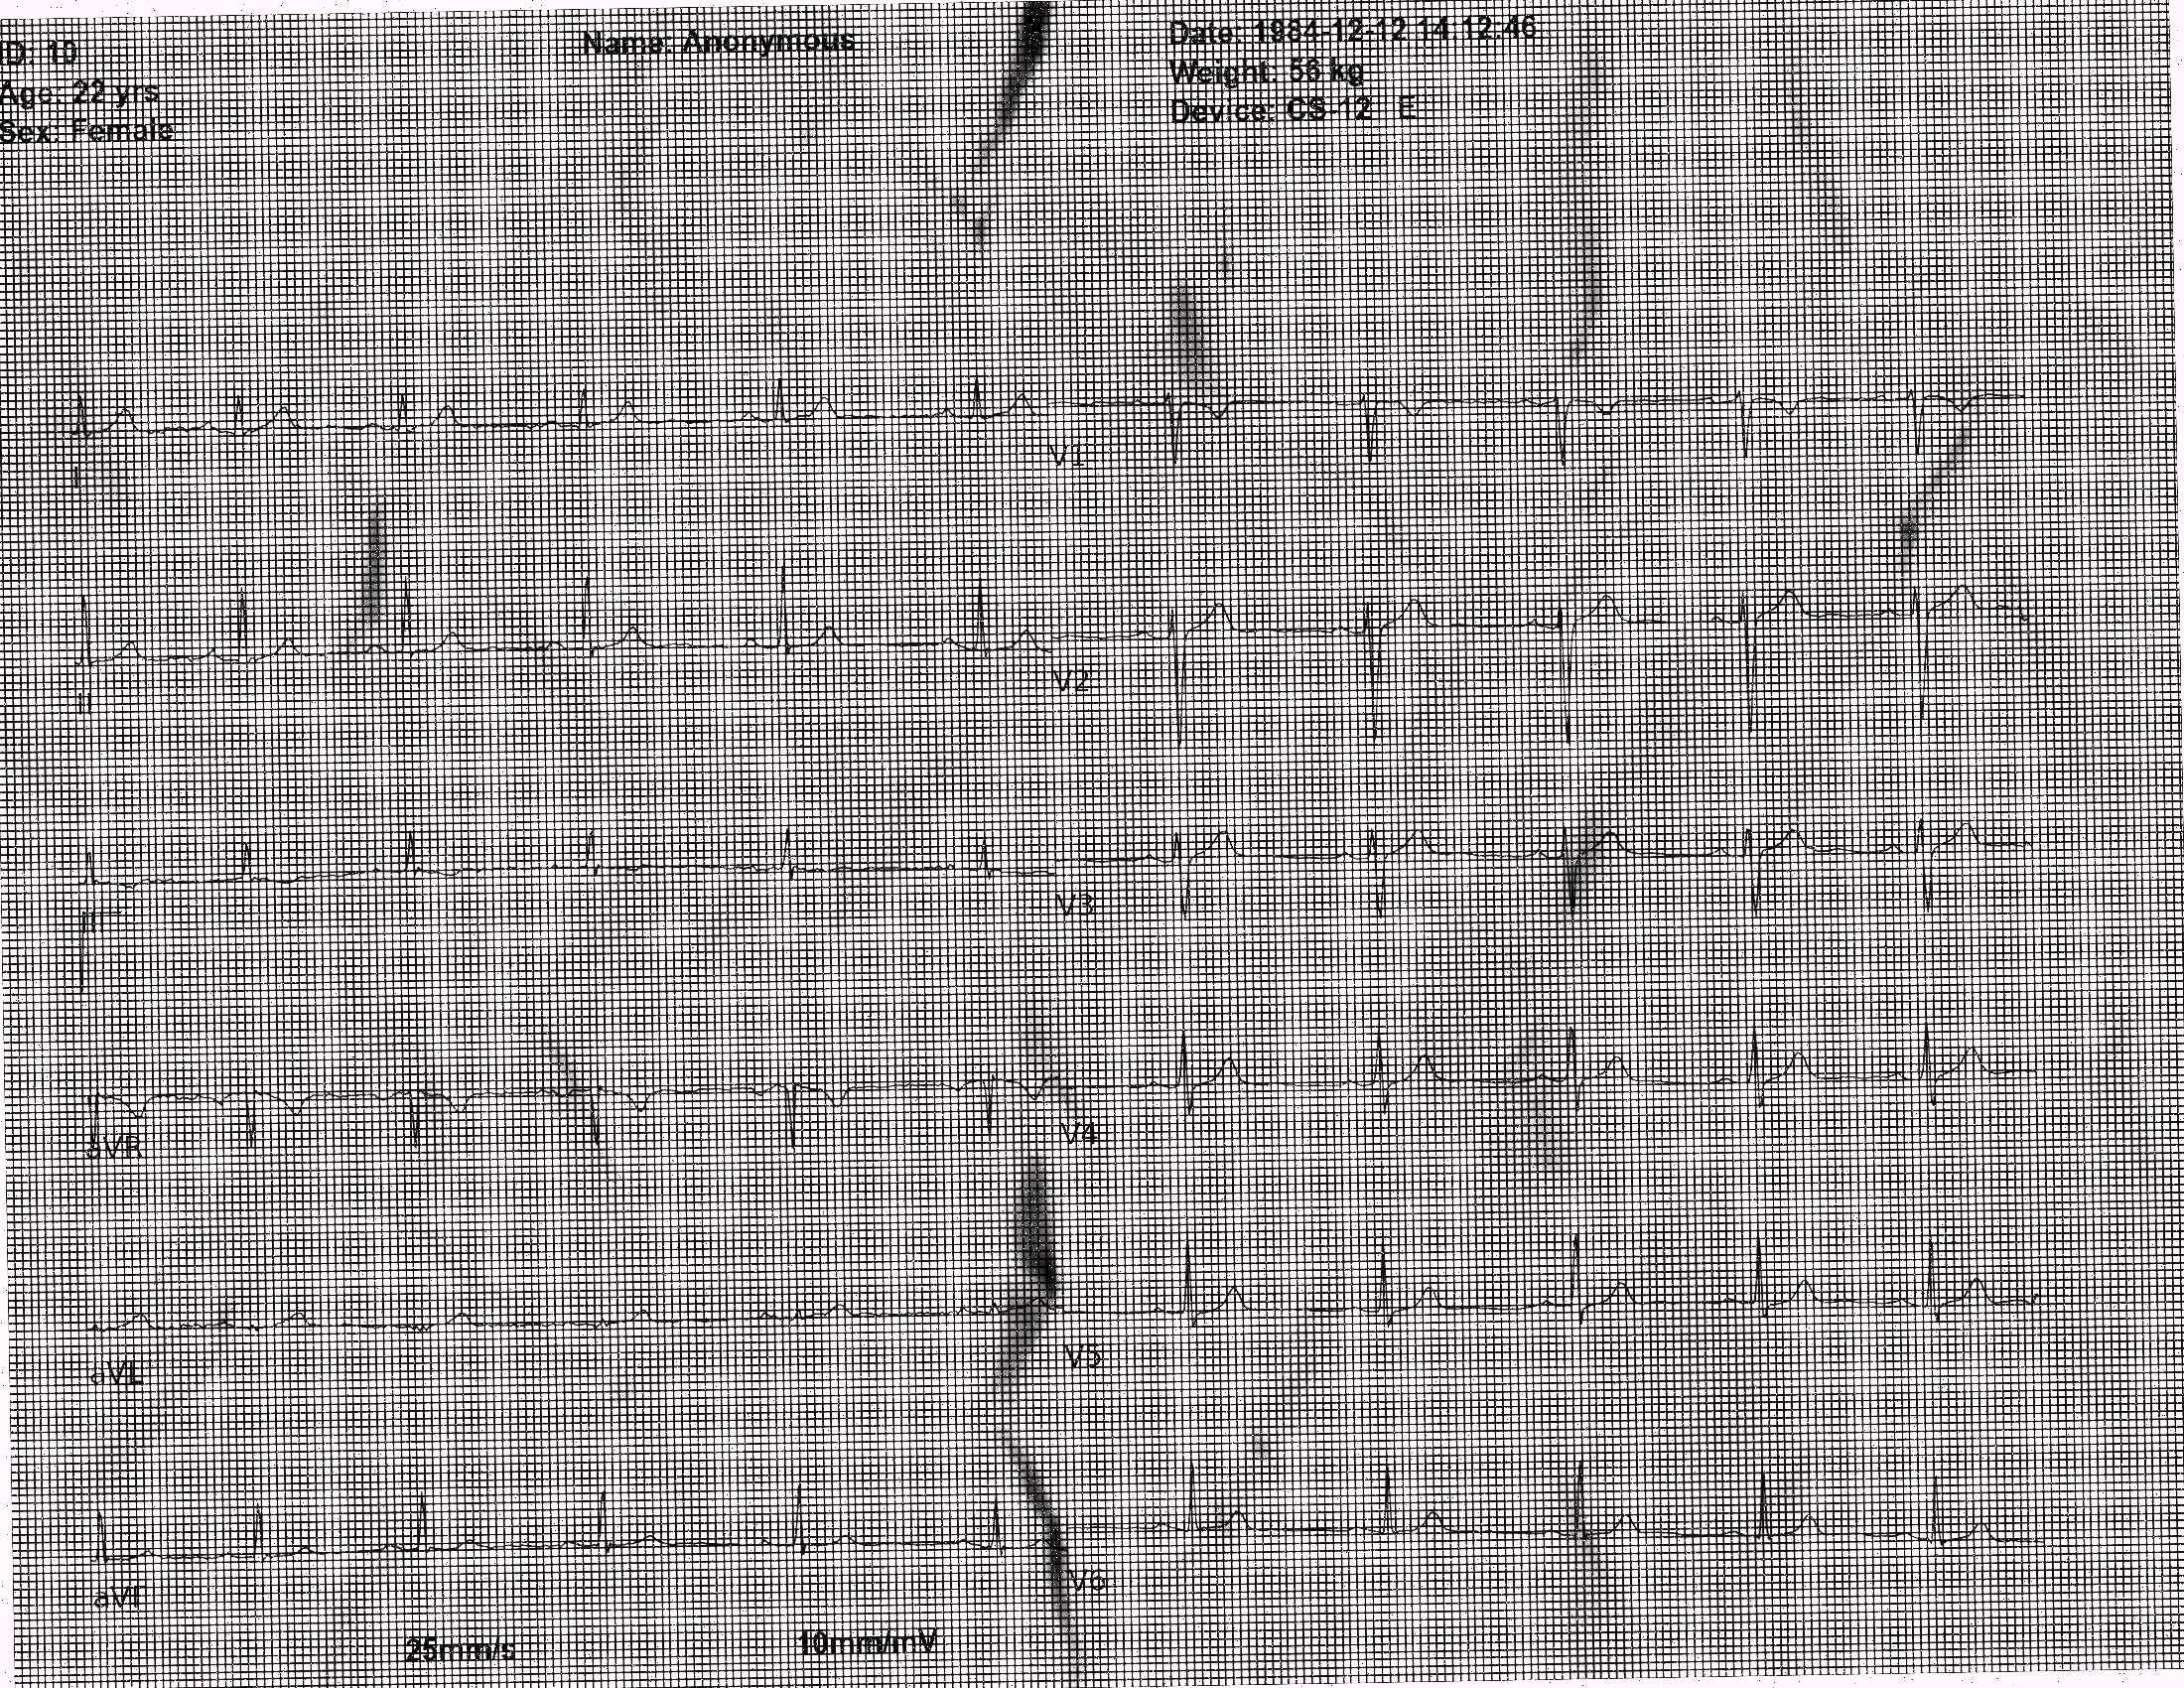
\includegraphics[width=0.7\textwidth, keepaspectratio]{images/augmented_plot.png}
    \caption{Output finale: applicazione di rumore, distorsioni geometriche e altri artefatti per la simulazione di documenti storici.}
    \label{fig:augmented_plot}
\end{figure}

\subsection{Logica di Rendering}
La trasformazione dal segnale digitale alla rappresentazione grafica è gestita da un motore di generazione basato su librerie di visualizzazione scientifica, configurato specificamente per garantire una corrispondenza millimetrica tra il segnale originale e i pixel del canvas. Tale precisione è fondamentale affinché la risoluzione spaziale risulti conforme agli standard clinici di riferimento. Il sistema opera con una risoluzione di rendering predefinita, ma permette una parametrizzazione flessibile dei parametri grafici per adattare l'output a diverse esigenze di analisi o di simulazione.
\vspace{4mm}

Nel prossimo capitolo, verrà analizzata l'architettura del sistema, descrivendo nel dettaglio le fasi di acquisizione dei dati, la configurazione del motore di rendering e l'implementazione tecnica della pipeline di degradazione.
